\chapter{Design \& Implementation}\label{sec:impl}

\section{Bitwidth analysis}
The analysis is built as a fixed point iteration using a lattice. After the analysis each operation has a $(int,boolean)$ tuple attached. 
The first value indicates the number of stable digits. 
The second value indicates if the output of the node is guaranteed to be positive. 
This flag is only meaningful when the mode of the corresponding node is signed. 
The boolean flag is especially useful for conversion optimization. A conversion from signed to unsigned can be analyzed more accurately. 
The lattice is described in \ref{fig:lattice}
\begin{figure}
	\centering
	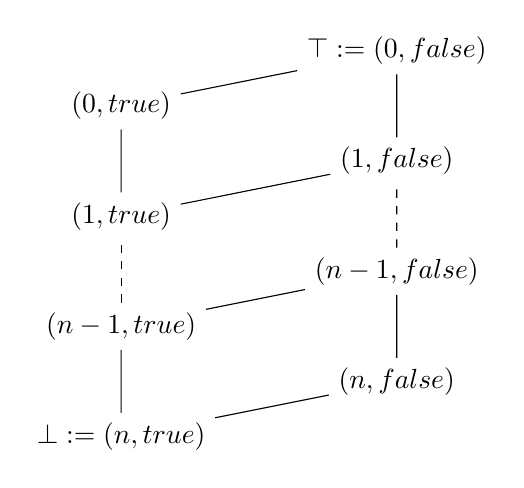
\begin{tikzpicture}[scale=.7]
		\node (np0) at(0,0) {$\bot := (n,true)$};
		\node (np1) at(0,2) {$(n-1,true)$};
		\node (np2) at(0,4) {$(1,true)$};
		\node (np3) at(0,6) {$(0,true)$};
		\node (p0) at(5,1) {$(n,false)$};
		\node (p1) at(5,3) {$(n-1,false)$};
		\node (p2) at(5,5) {$(1,false)$};
		\node (p3) at(5,7) {$\top := (0,false)$};
		\draw (np0) -- (p0) -- (p1) -- (np1) -- (np0);
		\draw (np2) -- (p2) -- (p3) -- (np3) -- (np2);
		\draw [dashed] (np1) -- (np2);
		\draw [dashed] (p1) -- (p2);
	\end{tikzpicture}
\caption{The definition of a upper bound compare node}
\label{fig:lattice}
\end{figure}

As a first step we iterate over every single node and initialize the node with $\top$ and mark them as \textit{dirty}. However, we safe one iteration for constant nodes by calculating them already in the first step. Nodes with the opcodes for \textit{Const}, \textit{Size} and \textit{Address} are considered constant.

The second step consists of recalculating every \textit{dirty} node in the graph. In case that $node.bitwidth > computed\_bitwidth$, the computed bitwidth is memorized as new bitwidth of the node and every successor of the node is marked as dirty. The rules that are used to recalculate the nodes are described in %TODO.

The tuple is defining a range of possible values. The exact range is depending on the mode of the node. Lets take the tuple $(stable\_digits,is\_positive)$
\begin{center}
	\begin{tabular}{| l | l | l |}
		\hline
		sign & min & max \\ \hline
		$true$ & $2^{stable\_digits-1}$ & $2^{stable\_digits-1}$-1. \\ \hline
		$false$ & 0 & $2^{stable\_digits}$-1 \\
		\hline
	\end{tabular}
\end{center}

\subsection{Value prediction}
In addition to the normal analysis results, the fixed point iteration can calculate upper and lower bounds for true and false blocks. However, this only works for compare nodes that are defining a upper bound. \newline
A compare node is defining a upper bound if $node.relation = <$ and the node at $node.right$ is constant. If this is the case then $\omega := node.left$ and the true block is called $\iota$. A visualization of the definition is given at \ref{fig:compare_upper_bound}.
\begin{figure}
	\centering
	\begin{tikzpicture}[scale=1.0, transform shape]
	\node[graph]{
		\begin{tikzpicture}[remember picture]
		\node[block] (startblock) {
			\begin{tikzpicture}
			\node[firm]    (predessors)       at (-1,3) {First};
			\node[firm]    (c2)       at ( 1,3) {Second};
			\node[firm]    (cmp)        at ( 0,2) {Cmp};
			\node[control] (cond)       at ( 0,1) {Cond};
			\node[control] (false)      at (-1,0) {Proj};
			\node[control] (true)       at ( 1,0) {Proj};
			
			\draw[dataDependency]    (cmp.120)     -- ++(0,0.1) -| (predessors);
			\draw[dataDependency]    (cmp.60)      -- ++(0,0.1) -| (c2);
			\draw[dataDependency]    (cond)        --              (cmp);
			\draw[controlDependency] (false.north) -- ++(0,0.1) -| (cond.240);
			\draw[controlDependency] (true.north)  -- ++(0,0.1) -| (cond.300);
			\end{tikzpicture}
		};
		\node[block, anchor=north east] (left) at ($(startblock.south) + (-1,-0.5)$) {
			\begin{tikzpicture}
			\node[const] (c0) at (0,0) {true-block};
			\end{tikzpicture}
		};
		\node[block, anchor=north west] (right) at ($(startblock.south) + (1,-0.5)$) {
			\begin{tikzpicture}
			\node[const] (c1) at (0,0) {false-block};
			\end{tikzpicture}
		};		
		% Control dependencies
		\begin{scope}[every path/.style = {controlDependency}]
			\draw (left.north)  -- ++(0,0.2) -| (false);
			\draw (right.north) -- ++(0,0.2) -| (true);
		\end{scope}
		
	\end{tikzpicture}
};
\end{tikzpicture}
\caption{The definition of a upper bound compare node}
\label{fig:compare_upper_bound}
\end{figure}

\newline
A compare node is also defining a upper bound if it can be transformed into a construct that matches the definition. For example with switching the right and left nodes, while turning the relation. \newline
For later usage we define the following 
\begin{center}
$\phi(a, b) := \forall X \prec a \wedge X.block = b$ 
\end{center}
$\phi$ returns every node that is a direct predecessor of a and located in block b.
\begin{center}
$\xi(a) := 
\left\{
	\begin{array}{l}
		a \cap \xi(c)\\ 
		\emptyset
	\end{array}
	\begin{array}{l}
		, \text{If there is only one not constant dependency \textit{c}} \\ 
		, \text{otherwise}.
	\end{array}
\right.$
\end{center}

If \textit{a} has only one not constant dependency node c, then $\xi$ returns the element a and $\xi(c)$. Otherwise it returns a empty set.

\paragraph{Upper bounds for block execution}
The values that are calculated in a node are (even if the fixed point iteration is not stable yet) possible values. The iteration starts at $\top$ and moves into the direction of $\bot$. This means that our range of possible values starts at something like $[0,0]$, moving towards $[n,-n]: n > 0 n <= max(mode)$ with each iteration. For a $\omega$ node this means that there can be a a recalculation, (new and old bitwidth is notated as the value range $\hat{x}$ and $x$) where the compare relation is true for $x$ but not anymore for  $\hat{x}$. This means that $\hat{x}$ is the upper bound for $\iota$. Thus we can insert a confirm node between every node $e \in \phi(\omega, \iota)$ and $\omega$.

\paragraph{Moving upper bounds backwards}
The confirms we have inserted between $\omega$ and its successors are not the only thing we can insert. We can also insert a confirm node between every $\phi(\xi(\omega), \iota)$. Important here is, the predecessors of $\omega$
Those confirms are then also inserted above conversation nodes, which is not possible using the normal construct insertion code provided by \libFIRM


\subsection{Difference to VRP}

There is already a analysis that is doing something similar, it is called value range propagation. The difference from VRP to BA is that in VRP each iteration is trying to predict the exact range after each operation. While BA tries to predict the unused bits after each operation. This little detail is mainly showing up in speed of the fixed point iteration, VRP converges way slower than BA. Details for this are given in the evaluation chapter \ref{sec:eval}.

\section{Stable Conversion nodes}
A conversion of a data word can result in two different results. First the bitwise representation stays the same. Second, the bitwise representation also gets mapped.
We call the first case \textit{Stable Conversion node}.

\paragraph{Finding stable conversion nodes}
Stable conversion nodes can be found using the bitwidth analysis. As described before, the analysis maps every node in the tree to a tuple. First number is the number of stable bits, which describes a upper bound for the numbers that will be written into the data word. The second number is a boolean flag and indicates if the number is going to be greater than 0 or not. If we now can see that the number range from the successor is the same as the one of the conversion node, then we can declare the conversion as stable.

\paragraph{Removing conversion nodes}
In case we found a stable conversion node, then we can say that this node only exists for syntax rules, there is no semantical value in them. Removing those nodes also has the advantage of helping other analysis. The confirm insertion algorithm of \libFIRM is searching for assertions that can be made based on looking at compare nodes. This works quite well. However, a construction like TODO does not work.
%FIXME diagram 
%FIXME reason
After removing the conversion node, the analysis can find a assertion based on the compare node. This also helps the branch prediction, dead code elimination. \newline
However, for really removing the conversion nodes, we need to find situations where we can eliminate the conversion node. One was already seen in the example. A compare node with a constant node as second operand. Another situation is a arithmetical operation with a constant and conversion node as operands.

\paragraph{Compare-Conversion optimization}
%FIXME diagram
\paragraph{Arithmetical-Conversion optimization}
%FIXME diagram